

\documentclass[12pt]{article}%
\usepackage{amsmath}%

%\usepackage{bibentry}%
\usepackage{amsfonts}%
\usepackage{amssymb}%
\usepackage{setspace}%
\usepackage{bbm}%
%\usepackage{harvard}
%\usepackage{chicago}
%\bibpunct[,~]{(}{)}{;}{a}{}{,}
\usepackage{enumerate}%
\usepackage{xfrac}
\usepackage[top=1in, bottom=1in, left=1in, right=1in]{geometry}
\usepackage{multirow}
\usepackage{rotating,graphicx}
\usepackage{subcaption}
\usepackage{caption}
\usepackage{rotating}
\usepackage{booktabs}
\usepackage[flushleft]{threeparttable}
\usepackage{subcaption}
\usepackage{float}
\usepackage{appendix}
\usepackage{titletoc}
\usepackage{rotating}



\usepackage[bookmarks=false,colorlinks=true, linkcolor=black, urlcolor=black, citecolor=black]{hyperref}

\usepackage{fullpage}

\usepackage{titlesec}

\usepackage[comma,longnamesfirst]{natbib}%

\newtheorem{hypothesis}{Hypothesis}
\usepackage{xcolor}

\usepackage{xr}

\pdfminorversion=6
\bibpunct[,~]{(}{)}{;}{a}{}{,}
\bibliographystyle{apsr}

\begin{document}
	
	\pagenumbering{arabic}
	\begin{doublespace}


\section*{Appendix A - Survey Questions}
Subjects were shown two applicants for state aid with the following prompt:

``Researchers have been hired to consult with a nearby state’s welfare agency. Below you will find two applicants for government assistance. The application information has been redacted to hide information that may identify individual applicants.

Each applicant has a state-assessed level of need of \$900 per month. \textbf{Your task is to allocate \$1,500 between the two applicants. You can allocate any amount between \$0 and \$900 to each applicant. Any remaining funds will be used to offset the state’s budget deficit.}"

Respondents were given three sliding scales to allocate funds. They could slide the bars or type numbers into the boxes on the right. At the bottom of the screen, the total amount they had awarded was shown relative to the full \$1,500 they had to distribute.

\begin{figure}[h!]
	\centering
	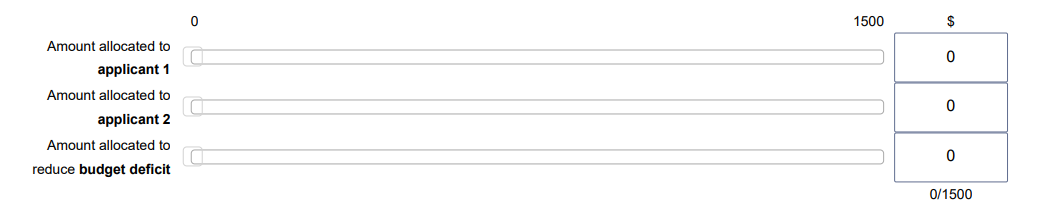
\includegraphics[scale=1]{figs/sliding-scale.png}
	\caption{Sliding Scale Used by Respondents to Make Allocations}
	\label{}
\end{figure}

\clearpage
\section*{Appendix B - Preregistration}

The analysis choices reported in the main text and our research hypotheses were pre-specified in the preregistration. We report our preregistration in this section. There are no departures from the pre-analysis plan. Some exploratory analysis is included in the main text and is denoted as such with a footnote. This experiment was Study 4 in a larger, grant-funded study, all of which was preregistered. As a result, the sections of the pre-registration relevant to this work are included.

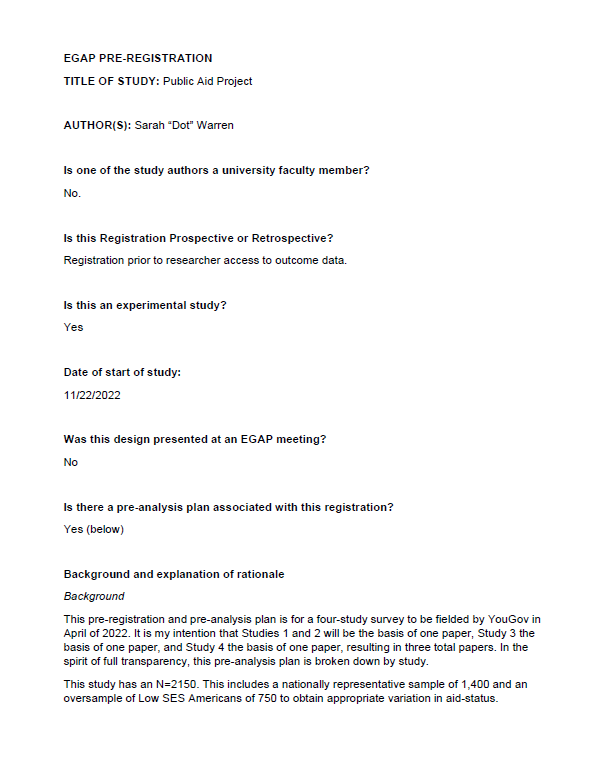
\includegraphics[scale=1.5]{figs/pap1.png} \\
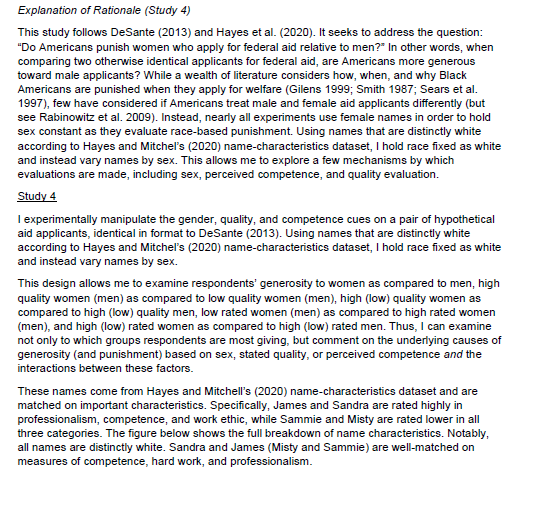
\includegraphics[scale=1.5]{figs/pap2.png} \\
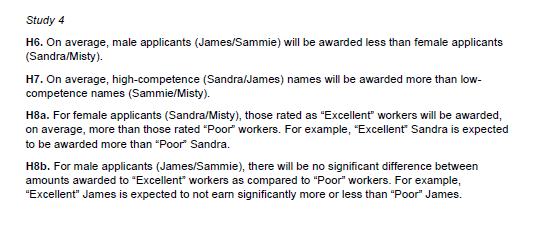
\includegraphics[scale=1.5]{figs/pap3.png} \\
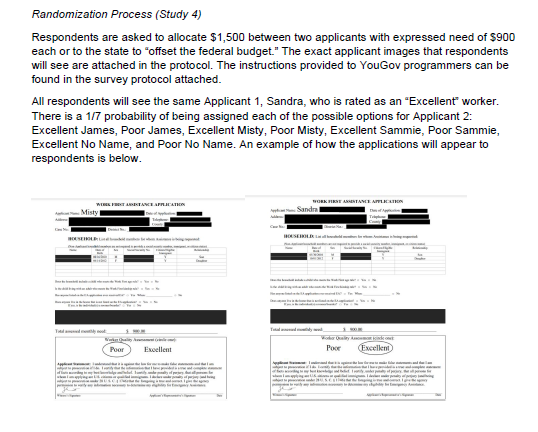
\includegraphics[scale=1.5]{figs/pap4.png} \\
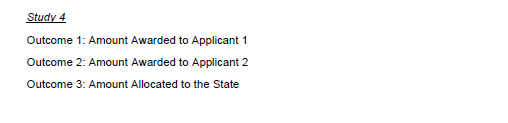
\includegraphics[scale=1.5]{figs/pap5.png} \\
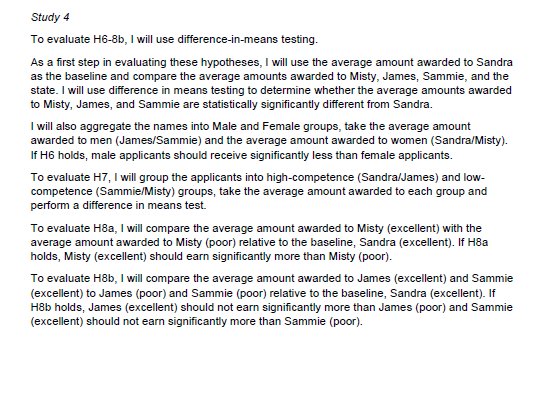
\includegraphics[scale=1.5]{figs/pap6.png}

\clearpage
\section*{Appendix C - Discussion of Ethics}

This research was reviewed and deemed exempt from review by the [redacted] Institutional Review Board. The experiment was programmed and conducted by YouGov, a large survey firm in the United States. Adult subjects ($>18$ years old) were drawn from a database of survey participants maintained and recruited by YouGov. There are no physical, psychological, social, or legal risks beyond the most minimal risks associated with everyday activity. In terms of economic or financial risks, subjects are paid and recruited by YouGov. Subjects do not pay to participate in the recruitment pool and no aspect of the survey or experiments therein require subjects to wager, bet, or contribute financially in any way. Thus, there are no reasonably foreseeable risks related to the subjects' participation in the experiment. No identifying information was shared to the researcher by YouGov. De-identified data were stored electronically on the researchers' server. There was no anticipated expiration of the data storage period. The de-identified data are available for purposes of replication once the research is published.





\end{doublespace}

\end{document}




